\cite{ARCADIA-Pancheri}
\cite{ARCADIA-Pancheri2}


ARCADIA (Advanced Readout CMOS Architectures with Depleted Integrated sensor Arrays) and SEED (Sensor with Embedded Electronic Developement) are both groups involved in the development of MAPS sensors based on the CMOS technology and both having LFoundry as industrial partner.
Many concept and performances studies have been carried out with simulations and small-scale test structure by SEED, before ARCADIA, applaying the experience developed with SEED to a full chip prototype, the MD1.  
MATISSE is an example of small-scale prototypes produced for testing: it is made by 24$\times$24 pixels organised in 4 columns; each pixel has an analog output, which allows for energy loss measurements, and a shutter snapshot readout with a speed that can reach \SI{5}{MHz}. 

The ARCADIA target are the development of a novel CMOS sensor platform allowing for fully depleted active sensors with thickness in range \SIrange{50}{500}{\um}. A small charge collecting electrode to achieve a good signal to noise ratio, a high time resolution (the lower bound is set at O(\si{\um}) but more advanced solutions are investigating for a O(\SI{10}{ns})) and a scalable readout architecture with low power consumption are the main requirement imposed by ARCADIA; the Main Demonstrator 1, has been submitted in 2020, and its characteristic are shown in table \ref{tab:ARCADIA_MD1}.
A second main demonstrator (ARCADIA-MD2) has been submitted in Summer 2021, featuring a similar design of MD1 and which is expected to be faster and to have a lower power consumption thanks to a logic and buffering optimisation. 

\begin{table}
    \begin{center}
    \begin{tabular}{| c |c |}
    \hline
    Parameter & Value\\
    \hline
    \hline
    Matrix size &  $\times$ \si{cm\squared}\\
    Pixel size & 25$\times$25 \si{\um\squared}\\
    Depth &  48/100/200\si{\um}\\
    Electrode size & 9$\times$9\si{\um\squared}\\
    Power consumption & $\sim$ 10\si{mW/cm\squared}\\    
    \hline
    \end{tabular}
    \caption{}
    \label{tab:ARCADIA_MD1}
    \end{center}
\end{table}

\section{The sensor and the front end}
    ARCADIA-MD1 is an LFoundry chip which implements the CMOS technology in 110 nm \ref{articolo fully depl}.
    The standard p-type substrate is replaced by a n-type \red{?}
    \begin{figure}[h!]
        \centering
        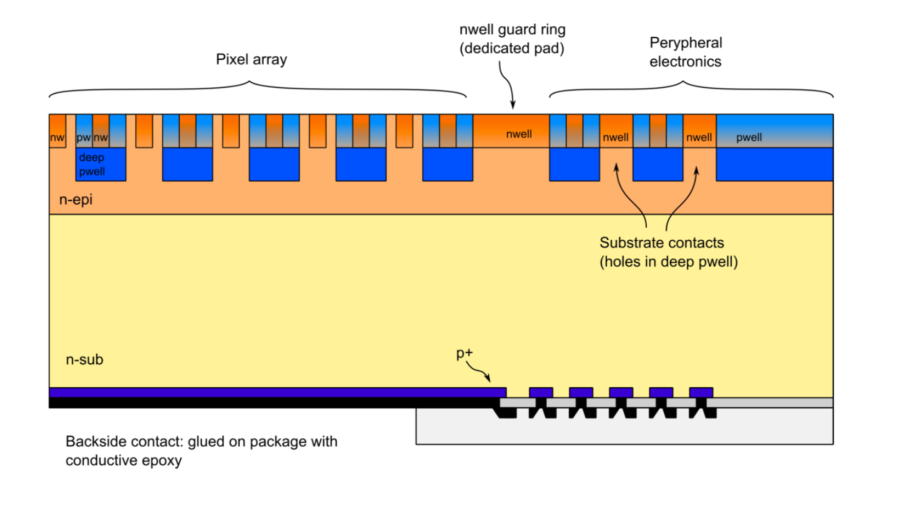
\includegraphics[width=.8\linewidth]{figures/ARCADIA/sensor.png}
        \caption{}
        \label{fig:ARCADIA_substrate}
    \end{figure}

    The sensor is made by a $p$ substrate and an $n$ doped diode within a $n$ epitaxial layer. 
    Being part of DMAPS cathegory, it is operated in fully depletion and the charge is then fastly collected by drift. 
    Up to now the sensor has been implemented in three different variant: \SI{48}{\um}, \SI{100}{\um} and \SI{200}{\um} thick, each with the same FE and readout logic but requiring a diffent biasing.  

        MD1 chips have been sumbitted in two different front end options: they are commonly called ALIPDE-like and bulk-driven.  
        The differences between them are in the FE circuit and in the biasing current of the registers, while the underlying readout is the same.
        The main difference is in the amplification stage, while in the ALPIDE-like flavor the amplification is implemented as explained in section \ref{sec:ALPIDE-like}, in the bulk-driven flavor the gain is adjusted by the ratio of two transconduttances. Consequently, some of the biasing registers, whose current is settable externally by the DAQ, have different default values and they might not be available at all in one of the flavor.
        An example is the ICLIP register, which is available only in the bulk driven flavor despite the transistor to which refers is implemented in both the flavor; its function is similar to the \emph{curfeed} capacitor in figure \ref{fig:Monopix1_FE_circuit}(a), which controls the current in the input branch of the FE and also influences the value of tha baseline at the discriminator input. 
        
        There are three types of configuration registers which are used to configure the matrix: 
        \begin{itemize}
            \item the Pixel Configuration Register, which is a 2-bits word used for enableling respectively the masking and injection functionalities. %Each bit is made by a latch which occupy \SI{14.560}{\um\squared} out of the per-pixel area available, \SI{205.72}{\um\squared}\footnote{\red{Perchè così? togli l'elettrodo e poi togli cos'altro?}}, then it is clear that there is not much extra space for any more configuration bits. 
            The on pixel Pixel Configuration Register circuit and how the mask/injection can be enable/disable is shown in figure \ref{fig:pixel_cfg}.
            \item the Internal Configuration Register, which are used for the comunication with the FPGA, for example to send a pulse, reset or configure the whole matrix.
            \item the Global Configuration Registers, which are used to set the configuration of the FE parameters are similar to the one of the TJ-Monopix1 circuit.
        \end{itemize}
        Their bias with the one of the sensors are supplied by padframes (a top, a bottom and a side one) placed aside the matrix, which also provide the clock, the reset, the test pulse for the injection circuit and the comunication signals.
        \begin{figure}[h!]
            \centering
            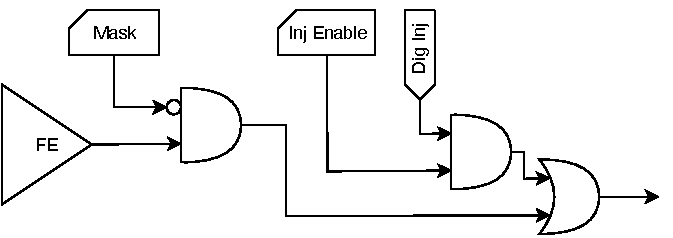
\includegraphics[width=.7\linewidth]{figures/ARCADIA/pixel_cfg.pdf}
            \caption{}
            \label{fig:pixel_cfg}
        \end{figure}    
        %Inoltre ci sono altre differenze, il bulk driven è più sensibile alle cadute di tensione sul ground (che ahimè è esattamente ciò che accade nei dimostratori che abbiamo ora, a causa dell'anomalo consumo di corrente dal digitale, altro baco che abbiamo corretto nella terza sottomissione).
        %Anche i livelli di tensione nei nodi interni dei due front-end differiscono e il meccanismo di clipping che funzionava per l'Alpide non è applicabile al bulk driven. Di conseguenza abbiamo un bias in più (ICLIP) nel secondo flavour per controllare il clipping. Nell'Alpide il clipping c'è, ma l'architettura usata permette di non aver bisogno di un bias esterno, anche se in una versione di Alpide di ALICE hanno scelto di controllare comunque la corrente di clip esternamente, per una maggiore flessibilità. Infine alcuni bias che hanno lo stesso nome nei due flavour, perché svolgono la stessa funzione, differiscono nel valore di configurazione didefault.
        %\begin{table}
        %    \begin{center}
        %    \begin{tabular}{|c | c | c |}
        %    \hline
        %    Parameter & Meaning & \\
        %    \hline
        %    \hline
        %    VCASD\\
        %    VINREF & provides the current to restore the input node i\\
        %    VCASN & set the threshold\\
        %    ICLIP\\
        %    IBIAS & discriminator current\\
        %    \hline
        %    \end{tabular}
        %    \caption{FE MD1 parameters which must be setted through the DAQ. "Function" means that higher parameter implies higher value}
        %    \label{tab:FE_ARCADIA-parameters}
        %%    \end{center}
        %\end{table}

\section{Readout logic and data structure}
    \subsection{Matrix division and data-packets}
    \begin{figure}[h!]
        \centering
        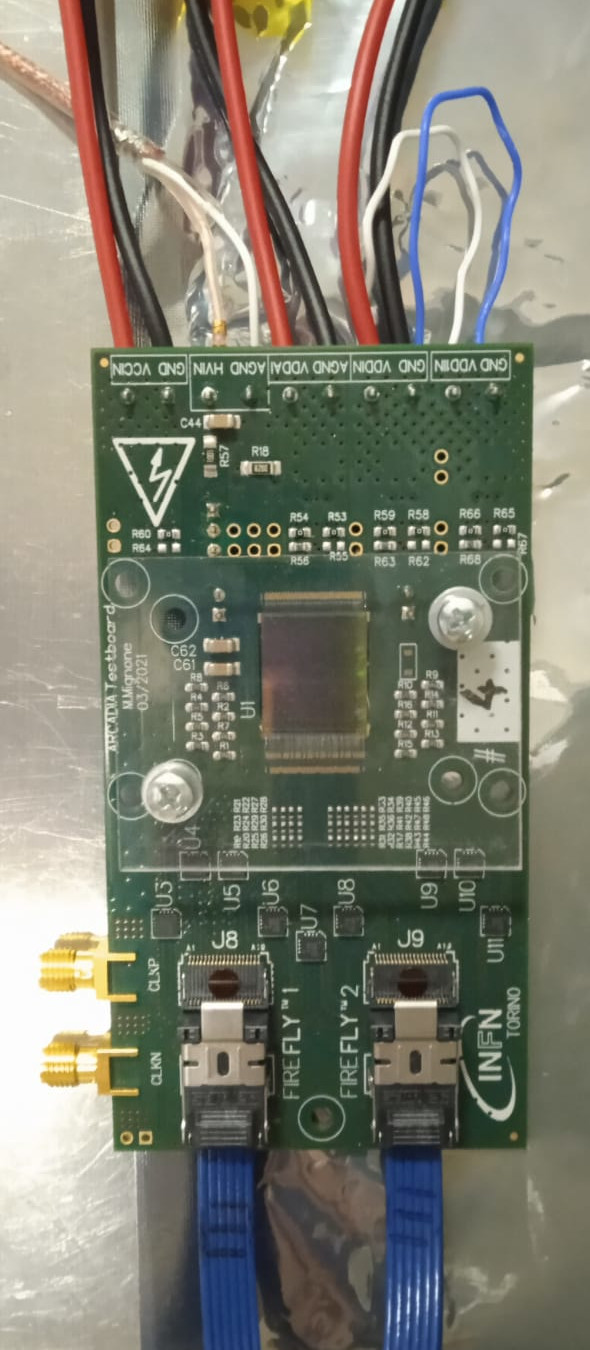
\includegraphics[width=.3\linewidth, angle =90 ]{figures/ARCADIA/arcadia_chip_front.jpeg}\\
        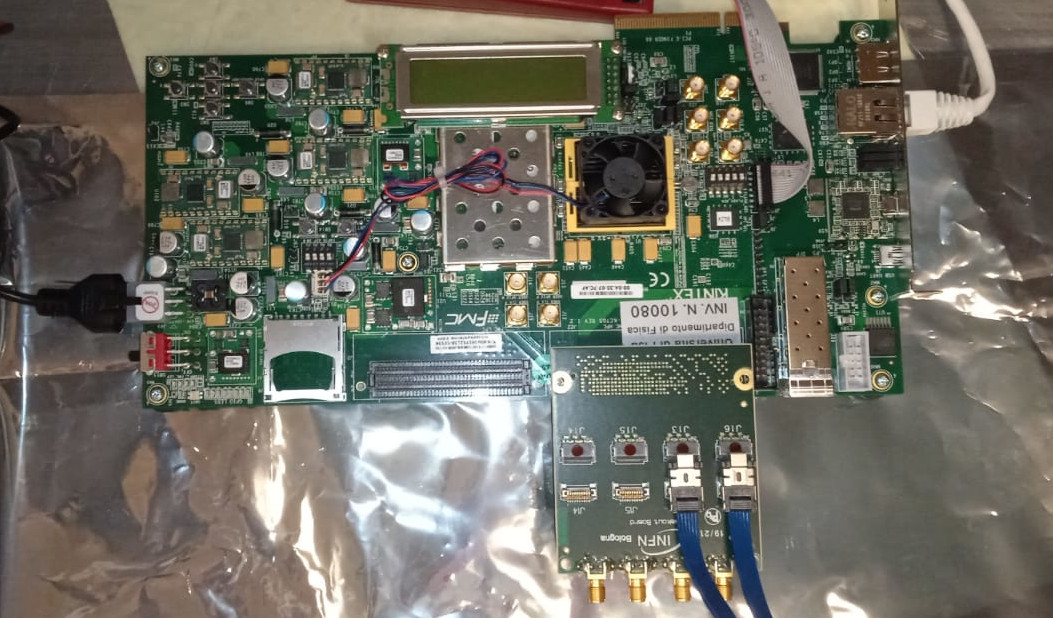
\includegraphics[width=.7\linewidth]{figures/ARCADIA/arcadia_FPGA.jpeg}
        \caption{(a) Board hosting the MD1 and (b) FPGA}
        \label{fig:}
    \end{figure}
    One of the main ambition of the MD1 is to achieve the lowest possible power consumption, hopefully less than \SI{20}{mW/cm\squared}; this is pricipally due to the hope of application also in space experiment field, where the power consumption and the cooling are for sure an issue. 
    In order to undergo that requirement, the matrix is clockless and the readout is triggerless; moreover the chip can be operated both in the high rate mode and low rate depending on if only one or all serializers, which are placed at the periphery of the matrix are enabled or only one is shared between the sections; in addition, to save as much area as possible, no buffer have been included on the matrix at the expense of the maximum hit rate sustainable. The readout then is completelly data push and when a hit is received immediately starts the readout mechanism to trasmit it off chip.

    The board hosting the chip is connected with a breakout board, which is connected to the FPGA; a data packet sent to the EoS, is then encoded and trasmitted to the FPGA using a \SI{320}{MHz} DDR serializers and then trasmitted by ethernet to the PC.
    %Sections with own 320MHz DDR Output link. The sections will have to have their own output link, in order to ease future up-scaling.-> lo dicono come requirement
    A photo of the experimental setup is shown in figure \ref{fig:photo}.

    \subsection{Matrix division and data-packets}
        \begin{figure}[h!]
            \centering
            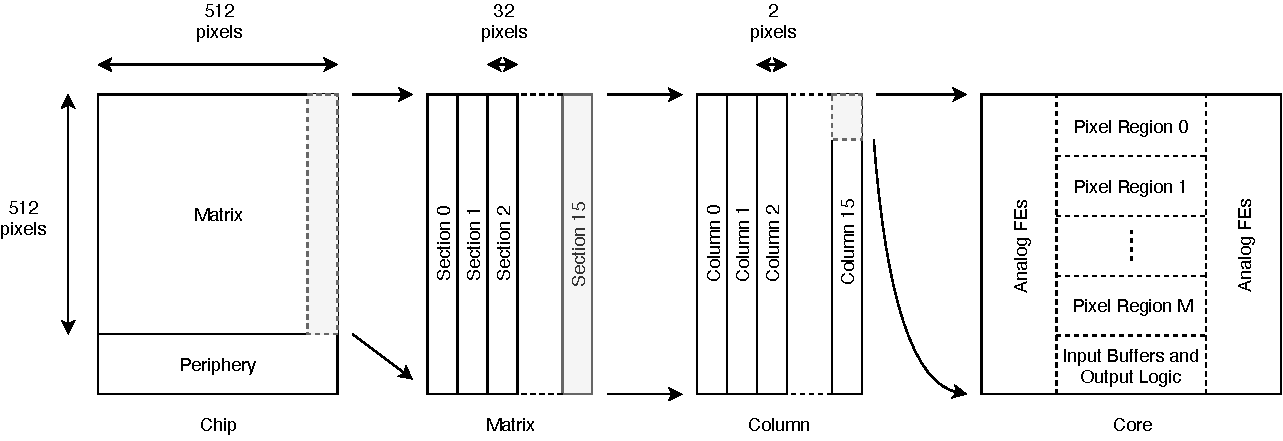
\includegraphics[width=.98\linewidth]{figures/ARCADIA/hierarchy.pdf}
            \caption{}
            \label{fig:hierarchy}
        \end{figure}
        Also the chip structure is meant to optimize the power consumption and the scalability for future up-scaling; in particular it is divide into a physical and logical hierarchy, which also reflects in the way the data pakets are built (tab.\ref{tab:data_packet}).
        First of all, the 512 columns are split in 16 sections each one containing 512$\times$32 pixels and having its own biasing lines and serializers at the matrix periphery. 
        Each section is is devided 512$\times$2 double-column mirrored, which just as in TJ-Monopix1, share the same readout buses placed between them and having analog logic on the sides.        
        The rows, then, are divided in group of 32, resulting in core with 32$\times$2 pixels. Finally each core is sub-divided in regions, each one containing 4$\times$2 pixels. 
        \begin{table}
            \begin{center}
            \begin{tabular}{|c |c |}
            \hline
            Bits & Meaning  \\
            \hline
            \hline
            31:24 & timestamp\\
            23:20 & section index\\
            19:16 & column index\\
            15:9 & pixel region\\
            8:0 & hitmap\\
            \hline
            \end{tabular}
            \caption{Data packet structure implemented by the MD1 readout logic.}
            \label{tab:data_packet}
            \end{center}
        \end{table}

        The readout has been designed with the constraints of being capable of handle with hit rate of \SI{100}{MHz/cm\squared}, then it has been optimized to minimize the amount of logic and to have a high bandwidth of trasmission of the data to the periphery. For this reason not all pixels have been provided by the readout logic.
        In particular, each pixel region can either be Master or Slave, depending on if has or has not the readout capability. 
        The Master's data packets are therefore composed of two parts: the hitmap of the Master itself and the one of Slave. 
        Moreover, the pioneer idea of ARCADIA-MD1, which has as finally goal the test of a readout cabable of transmit cluster data in as few data packets as possible, is the possibility of the Master to decide what Slave (top or bottom) read; the information of what Slave has been selected is represented by a bit, often called \emph{hot bit}, in the data-packet.
        Every pixel has an associated status register, that essentialy is a flip flop (FF), which is set to 1 when the pixel stores a hit; an OR of the FF whithin the Master or the Slave region generates an active flag which is used to require a readout by the EoS.  
        \begin{figure}[h!]
            \centering
            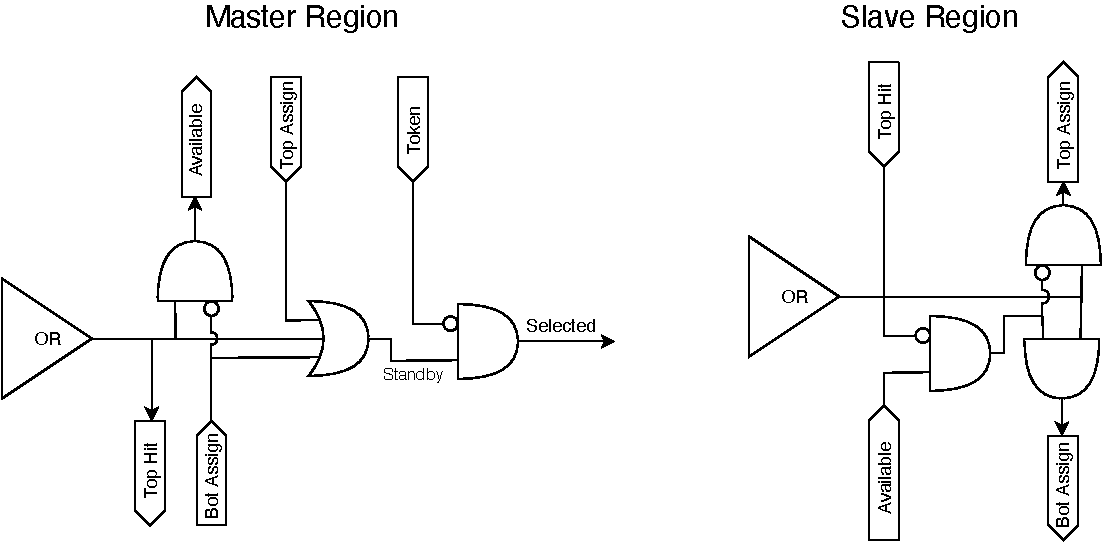
\includegraphics[width=.95\linewidth]{figures/ARCADIA/clustering_logic.pdf}
            \caption{}
            \label{fig:clustering_logic}
        \end{figure}
        In figure \ref{fig:clustering_logic} is shown the circuit with the logic of assignment of the Slave to the Master.
        

        Depending on the active flags of the neighbouring Masters, the Slave hitmap is assigned to the one at the top or bottom. 
        %\red{The circuit which does that is shown in figure \ref{fig:clustering_logic}}. 
        If both the Masters have an active flag, the Slave is assigned to the top one. 
        \begin{figure}[h!]
            \centering
            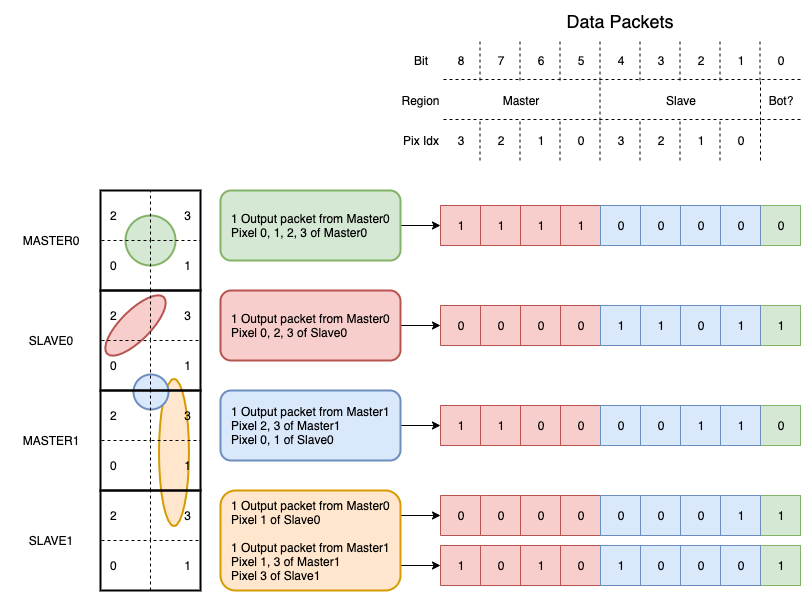
\includegraphics[width=.95\linewidth]{figures/ARCADIA/clustering.png}
            \caption{Different cluster structures and the data packet produced by them are shown in the example.}
            \label{fig:clustering}
        \end{figure}
        In the example in figure \ref{fig:clustering} two Master-Slave regions are considered: the hitmaps of the Master (red colored in the example) and Slave (blue colored) are joined together within a unique data packet and a bit (green colored) is used to specify the Slave. 

        The data packets are transmitted to the End of Section (EoS) with a priority chain similar to what happens in TJ-Monopix1. 
        If at least one Master set a high flag, a \textcolor{Cerulean}{Token} signal is generated and is assigned to the high priority Master in the column, together with a \textcolor{red}{Full} flag which is distributed to the active Masters in the whole column in order to deny more region to be accesed at the same time.
        The readout then propagates down the column from Master to Master, skipping the empy cores; the Master selected for the readout is the one with the flag high and with an input (from top) \textcolor{Cerulean}{Token} equal to 0. 
        In the example in figure \ref{fig:token_chain} the \textcolor{Cerulean}{Token} is propagated from the Pixel Region (PR) 10 to the PR 7. 
        In the three readout steps the red Masters are the ones selected for the readout, while the yellow are the ones which an active flag high; gray color is used for empty regions. When a specific Master has been selected, a \textcolor{Cerulean}{Read} signal is generated both to transmit the data to the EoS and also to generate a reset for the just read pixels.
        Once the pixels are reset, the Master's \textcolor{red}{Full} 
        and \textcolor{Cerulean}{Token} flags fall, and the following region which satisfys the two readout conditions explained above, becomes selected. 
        \begin{figure}[h!]
            \centering
            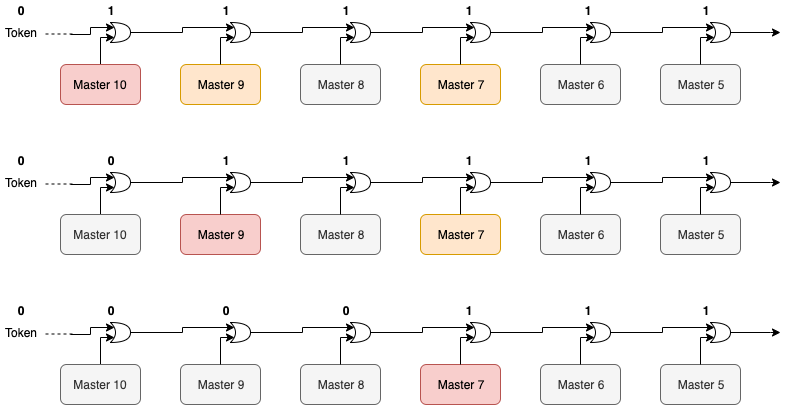
\includegraphics[width=.95\linewidth]{figures/ARCADIA/token_chain.png}
            \caption{}
            \label{fig:token_chain}
        \end{figure}

    The performances of the readout has been studied with simulations by the designer of the chip. 
    Random hits events with cluster size of 4 pixels on average, with a Poissonian distribution in time and uniformely distributed on the matrix has been generated.
    They state that with particle hit rate of \SI{100}{MHz/cm\squared}, considering a portion of matrix of three section (512$\times$96), the efficiency results to be 98.7\%, while reducing the hit rate to \SI{80}{MHz/cm\squared} it is even higher achieving the 99.95\%. 